\documentclass{article}

% Paquets nécessaires
\usepackage{amsmath} % Pour les mathématiques
\usepackage{amsfonts} % Pour les polices mathématiques supplémentaires
\usepackage{amssymb} % Pour les symboles mathématiques
\usepackage{tikz} % Pour les graphiques vectoriels
\usepackage{pgfplots} % Pour les graphiques en 2D et 3D
\usepackage{setspace} % Pour l'espacement des lignes
\usepackage{color} % Pour les couleurs de texte
\usepackage{mathrsfs} % Pour les lettres cursives en mathématiques
\usepackage{blindtext}
\usepackage{pdflscape}
\usepackage{adjustbox}
\usepackage{geometry}
\usepackage{xcolor}

\usetikzlibrary{automata, positioning, arrows}
% Configuration des bibliothèques TikZ
\usepgfplotslibrary{fillbetween}
\pgfplotsset{compat=1.18}

% Configuration de la page


\title{Devoir 3}
\author{Emeric Laberge,Sara Haddad}
\date{\today}
\begin{document}
\begin{titlepage}
   \begin{center}
      \vspace*{1cm}
                  
      \Huge
      \textbf{Devoir 3} 
                  
      \vspace{0.5cm}
      \LARGE
                  
      \vspace{1.5cm}
                  
      \textbf{Emeric Laberge}\\ 20220275 \\ \textbf{Sara Haddad} \\ 20208373
                  
      \vfill
                  
      Dans le cadre du cours\\
      IFT 1575
      
                  
      \vspace{0.8cm}
                  
      
\includegraphics[width=0.4\textwidth]{Université-de-Montréal.jpg}
                   
      \Large
      Département d'informatique et de recherche opérationnelle\\
      Université de Montréal\\
      Canada\\
      27 mars 2023
                  
    \end{center}
\end{titlepage}

\newgeometry{
    top=3cm,
    bottom=1.5cm,
    left=6cm,
    right=4cm,
}
\begin{landscape}
% \begin{center}
% \begin{table}[]
%     \begin{tabular}{|l|l|l|l|l|l|l|l|l|l|}
%         \hline
%         serveur & 1     & 2     & 3     & 4     & 5     & 6     & 7     & 8     & 9     \\ \hline
%         heures  & 17-21 & 13-19 & 16-19 & 18-22 & 19-23 & 13-17 & 18-23 & 17-23 & 13-21 \\ \hline
%         salaire & 68\$  & 90\$  & 38\$  & 61\$  & 56\$  & 60\$  & 63\$  & 105\$ & 120\$ \\ \hline
%     \end{tabular}
% \end{table}
% \end{center}
   \begin{center}
        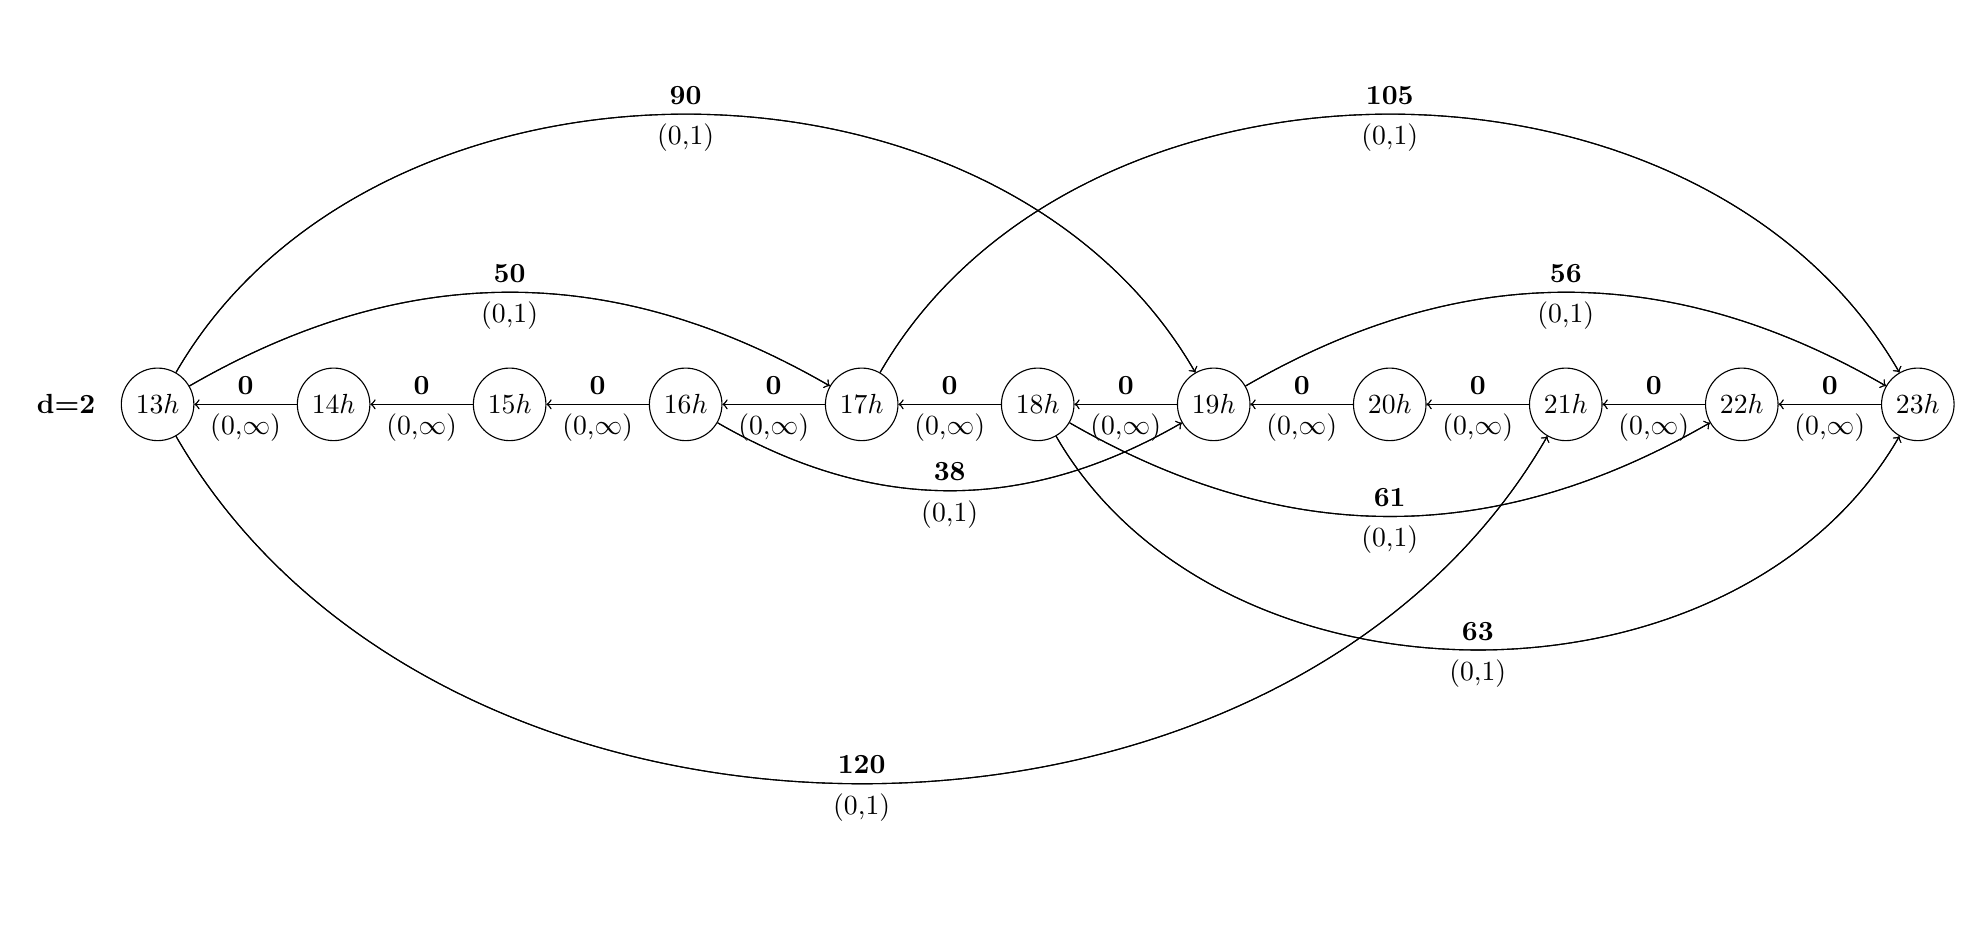
\begin{tikzpicture}[node distance=1.3cm,auto]
            \tikzset{label/.style={midway,font=\small}}

            \node[state] (13h) {$13h$};
            \node[state] (14h) [right = of 13h] {$14h$};
            \node[state] (15h) [right = of 14h] {$15h$};
            \node[state] (16h) [right = of 15h] {$16h$};
            \node[state] (17h) [right = of 16h] {$17h$};
            \node[state] (18h) [right = of 17h] {$18h$};
            \node[state] (19h) [right = of 18h] {$19h$};
            \node[state] (20h) [right = of 19h] {$20h$};
            \node[state] (21h) [right = of 20h] {$21h$};
            \node[state] (22h) [right = of 21h] {$22h$};
            \node[state] (23h) [right = of 22h] {$23h$};

            \node[left= 0.2cm of 13h] {\textbf{d=2}};


            % \node[state,accepting] (q1) [above right=of q0] {$q_1$};
            % \node[state,accepting] (q2) [below right=of q0] {$q_2$};
            % \draw[->] (q5) edge [bend right] node {0} (q3);
            % \draw[->] (q5) edge [loop above] node {1} ();

            \draw[->,align=center] (13h) edge [bend left,out=60,in=120] node[above] {\textbf{90}} (19h);
            \draw[->,align=center] (13h) edge [bend left,out=60,in=120] node[below] {(0,1)} (19h);


            \draw[->,align=center] (13h) edge [bend left] node[above] {\textbf{50}} (17h);
            \draw[->,align=center] (13h) edge [bend left] node[below] {(0,1)} (17h);

            \draw[->,align=center] (13h) edge [bend right , in=240,out=300] node[above] {\textbf{120}} (21h);
            \draw[->,align=center] (13h) edge [bend right , in=240,out=300] node[below] {(0,1)} (21h);

            \draw[->,align=center] (16h) edge [bend right] node[above] {\textbf{38}}  (19h);
            \draw[->,align=center] (16h) edge [bend right] node[below] {(0,1)} (19h);

            \draw[->,align=center] (17h) edge [bend left,out=60,in=120 ] node[above] {\textbf{105}} (23h);
            \draw[->,align=center] (17h) edge [bend left,out=60,in=120 ] node[below] {(0,1)} (23h);

            \draw[->,align=center] (18h) edge [bend right] node[above] {\textbf{61}} (22h);
            \draw[->,align=center] (18h) edge [bend right] node[below] {(0,1)} (22h);

            \draw[->,align=center] (18h) edge [bend left,out=300,in=240] node[above] {\textbf{63}} (23h);
            \draw[->,align=center] (18h) edge [bend left,out=300,in=240] node[below] {(0,1)} (23h);

            \draw[->,align=center] (19h) edge [bend left] node {\textbf{56}} (23h);
            \draw[->,align=center] (19h) edge [bend left] node[below] {(0,1)} (23h);





            \draw[->] (14h) edge node[above] {\textbf{0}} (13h);
            \draw[->] (14h) edge node[below] {(0,$\infty$)} (13h);

            \draw[->] (15h) edge node[above] {\textbf{0}} (14h);
            \draw[->] (15h) edge node[below] {(0,$\infty$)} (14h);

            \draw[->] (16h) edge node[above] {\textbf{0}} (15h);
            \draw[->] (16h) edge node[below] {(0,$\infty$)} (15h);

            \draw[->] (17h) edge node[above] {\textbf{0}} (16h);
            \draw[->] (17h) edge node[below] {(0,$\infty$)} (16h);

            \draw[->] (18h) edge node[above] {\textbf{0} }(17h);
            \draw[->] (18h) edge node[below] {(0,$\infty$)} (17h);

            \draw[->] (19h) edge node[above] {\textbf{0}} (18h);
            \draw[->] (19h) edge node[below] {(0,$\infty$)} (18h);

            \draw[->] (20h) edge node[above] {\textbf{0}} (19h);
            \draw[->] (20h) edge node[below] {(0,$\infty$)} (19h);

            \draw[->] (21h) edge node[above] {\textbf{0}} (20h);
            \draw[->] (21h) edge node[below]{(0,$\infty$)} (20h);

            \draw[->] (22h) edge node[above] {\textbf{0}} (21h);
            \draw[->] (22h) edge node[below] {(0,$\infty$)} (21h);  

            \draw[->] (23h) edge node[above] {\textbf{0}} (22h);
            \draw[->] (23h) edge node[below] {(0,$\infty$)} (22h);


        \end{tikzpicture}
    \end{center}
\end{landscape}

\restoregeometry

\clearpage
\section*{Question 2}
% \begin{center}
%     \begin{tikzpicture}[auto]
%         %\tikzset{label/.style={midway,font=\small}}
%         \node[state] (1) {1};
%         \node[state] (2) [above right = of 1] {2};

%         \node[state] (3) [below right = of 1] {3};
%         \node[state] (4) [below right = of 2] {4};
%         \node[state] (5) [above right = of 4] {5};
%         \node[state] (6) [below right = of 4] {6};
%         \node[state] (7) [below right = of 5] {7};

%         \draw[->] (1) edge node {\textbf{10}} (2);
%         \draw[->] (1) edge node[below left] {\textbf{25}} (3);
%         \draw[->] (1) edge node {\textbf{16}} (4);

%         \draw[->] (2) edge node {\textbf{5}} (4);
%         \draw[->] (2) edge node {\textbf{22}} (5);

%         \draw[->] (3) edge node[below] {\textbf{2}} (6);

%         \draw[->] (4) edge node {\textbf{15}} (5);
%         \draw[->] (4) edge node {\textbf{22}} (6);
%         \draw[->] (4) edge node {\textbf{7}} (3);

%         \draw[->] (5) edge node {\textbf{20}} (6);
%         \draw[->] (5) edge node {\textbf{10}} (7);

%         \draw[->] (6) edge node[below right] {\textbf{5}} (7);
%     \end{tikzpicture}
% \end{center}


\textbf{Initialisation:} \quad $EM=\{1\} \quad ; \quad  \delta_1=0$
\subsection*{Itération 1:}
\subsubsection*{Étape 1:}
Les successeurs de $1$ sont $2$, $3$ et $4$.\\
$\lambda_{12}=10 \quad \lambda_{13}=25 \quad \lambda_{14}=16$\\
min $\{\lambda_{12},\lambda_{13},\lambda_{14}\} = $ min$\{10,25,16\}=10 \Rightarrow j_1 =2 $\\
\subsubsection*{Étape 2:}
On détermine le chemin le plus court menant de $1$ à $j_1$\\
min $\{ \delta_1 + \lambda_{12}\} = $ min $\{0+10\}=10 $\\
marquer $j_1=2$ avec $\delta_2=10$\\ 
\subsubsection*{Étape 3:}
$EM \leftarrow EM \cup \{j_1\}$ \quad avec $ \delta_{21} = \delta_1 + \lambda_{12} = 10$ \\
$EM = \{1,2\}$\\
\subsubsection*{Étape 4:}
%make a bar above EM
$\overline{EM} \neq \emptyset $ , alors on effectue un autre itération
\begin{center}
    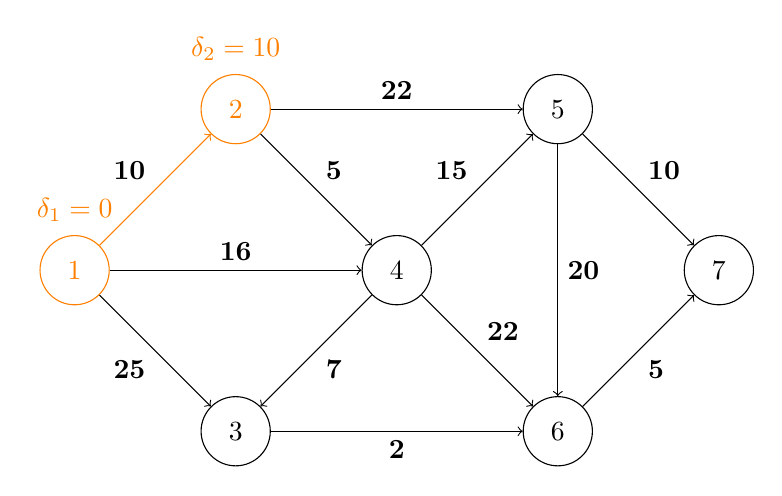
\begin{tikzpicture}[node distance = 2 cm , auto]
        %\tikzset{label/.style={midway,font=\small}}
        \node[state,color=orange] (1) {1};
        \node[above= 0.05 cm of 1] {\textbf{\textcolor{orange}{$\delta_1=0$}}};
        \node[state,color=orange] (2) [above right = of 1] {2};
        \node[above= 0.05 cm of 2] {\textbf{\textcolor{orange}{$\delta_2=10$}}};

        \node[state] (3) [below right = of 1] {3};
        \node[state] (4) [below right = of 2] {4};
        \node[state] (5) [above right = of 4] {5};
        \node[state] (6) [below right = of 4] {6};
        \node[state] (7) [below right = of 5] {7};

        \draw[->,color=orange] (1) edge[color=orange] node[color=black] {\textbf{10}} (2);
        \draw[->] (1) edge node[below left] {\textbf{25}} (3);
        \draw[->] (1) edge node {\textbf{16}} (4);

        \draw[->] (2) edge node {\textbf{5}} (4);
        \draw[->] (2) edge node {\textbf{22}} (5);

        \draw[->] (3) edge node[below] {\textbf{2}} (6);

        \draw[->] (4) edge node {\textbf{15}} (5);
        \draw[->] (4) edge node {\textbf{22}} (6);
        \draw[->] (4) edge node {\textbf{7}} (3);

        \draw[->] (5) edge node {\textbf{20}} (6);
        \draw[->] (5) edge node {\textbf{10}} (7);

        \draw[->] (6) edge node[below right] {\textbf{5}} (7);
    \end{tikzpicture}
\end{center}
\pagebreak

\subsection*{Itération 2:}
$EM = \{1,2\}$
\subsubsection*{Étape 1:}
On identifie le sommet adjacent non marqué situé le plus près de:
\begin{enumerate}
    \item min $\{\lambda_{13},\lambda_{14}\}=$ min $\{25,16\}=16\Rightarrow j_1=4$ \\
    \item min $\{\lambda_{24},\lambda_{25}\}=$ min $\{5,22\}=5\Rightarrow j_2=4$ \\
\end{enumerate}
\subsubsection*{Étape 2:}
min $\{ \delta_1 + \lambda_{14},\delta_2+\lambda_{24}\} = $ min $\{0+16,10+5\}=15 $\\
marquer le sommet $j_2=4$ avec $\delta_4=15$\\ 
\subsubsection*{Étape 3:}
$EM=\{1,2,4\}$
\subsubsection*{Étape 4:}
$\overline{EM} \neq \emptyset $ , alors on effectue un autre itération
%make a bar above EM
$\overline{EM} \neq \emptyset $ , alors on effectue un autre itération

\begin{center}
    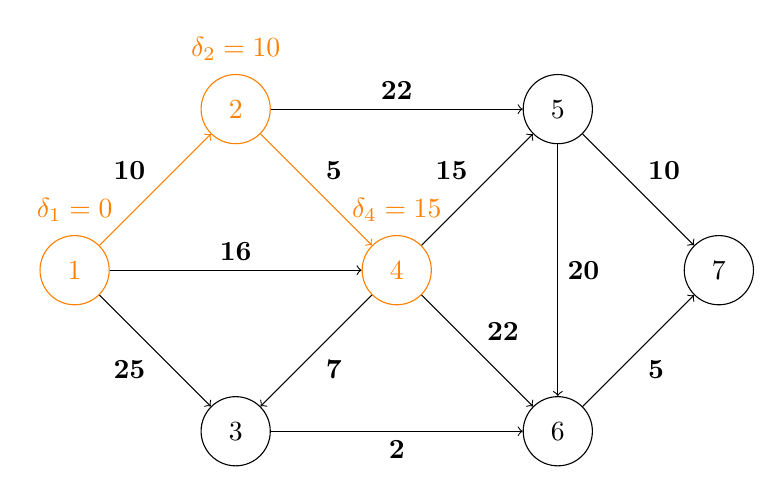
\begin{tikzpicture}[node distance = 2 cm , auto]
        %\tikzset{label/.style={midway,font=\small}}
        \node[state,color=orange] (1) {1};
        \node[above= 0.05 cm of 1] {\textbf{\textcolor{orange}{$\delta_1=0$}}};
        \node[state,color=orange] (2) [above right = of 1] {2};
        \node[above= 0.05 cm of 2] {\textbf{\textcolor{orange}{$\delta_2=10$}}};

        \node[state] (3) [below right = of 1] {3};
        \node[state,color=orange] (4) [below right = of 2] {4};
        \node[above= 0.05 cm of 4] {\textbf{\textcolor{orange}{$\delta_4=15$}}};
        \node[state] (5) [above right = of 4] {5};
        \node[state] (6) [below right = of 4] {6};
        \node[state] (7) [below right = of 5] {7};

        \draw[->,color=orange] (1) edge[color=orange] node[color=black] {\textbf{10}} (2);
        \draw[->] (1) edge node[below left] {\textbf{25}} (3);
        \draw[->] (1) edge node {\textbf{16}} (4);

        \draw[->] (2) edge node {\textbf{22}} (5);
        \draw[->,color=orange] (2) edge[color=orange] node[color=black] {\textbf{5}} (4);

        \draw[->] (3) edge node[below] {\textbf{2}} (6);

        \draw[->] (4) edge node {\textbf{15}} (5);
        \draw[->] (4) edge node {\textbf{22}} (6);
        \draw[->] (4) edge node {\textbf{7}} (3);

        \draw[->] (5) edge node {\textbf{20}} (6);
        \draw[->] (5) edge node {\textbf{10}} (7);

        \draw[->] (6) edge node[below right] {\textbf{5}} (7);
    \end{tikzpicture}
\end{center}

\pagebreak 

\subsection*{Itération 3:}
$EM = \{1,2,4\}$
\subsubsection*{Étape 1:}
On identifie les sommets adjacents non marqués situé les plus près de:
\begin{itemize}
    \item \textbf{(1)} min $\{\lambda_{13}\}=25 \: \Rightarrow j_1 =3$ \\
    \item \textbf{(2)} min $\{\lambda_{25}\}=22 \: \Rightarrow j_2 =5$ \\
    \item \textbf{(4)} min $\{\lambda_{43},\lambda_{45},\lambda_{46},\}=$ min $\{7,15,22\}=7 \: \Rightarrow j_4 =3$ \\
\end{itemize}
\subsubsection*{Étape 2:}
min $\{ \delta_1 + \lambda_{13}\: , \:\delta_4+\lambda_{43} \: ,\:\delta_2+\lambda_{25}\} = $ min $\{0+25 \:,\:15+7 \:,\:\}=22 $\\
marquer le sommet $j_4=3$ avec $\delta_3=22$\\ 
\subsubsection*{Étape 3:}
$EM=\{1,2,4,3\}$
\subsubsection*{Étape 4:}
$\overline{EM} \neq \emptyset $ , alors on effectue un autre itération

\begin{center}
    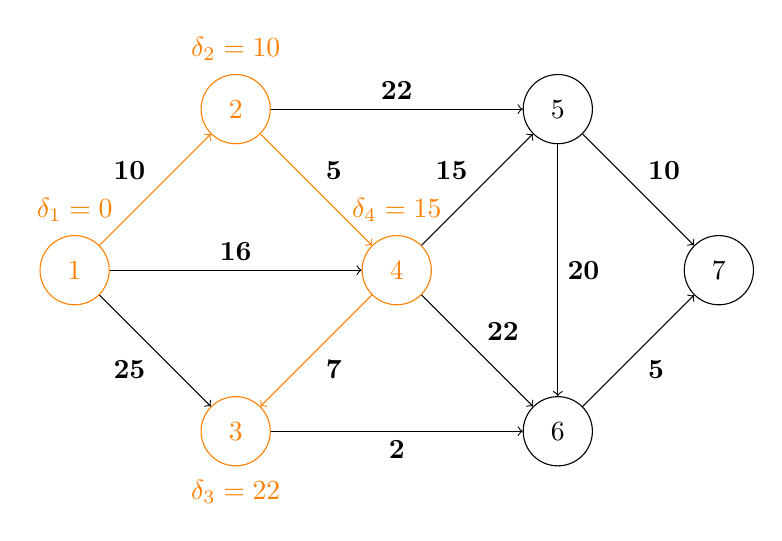
\begin{tikzpicture}[node distance = 2 cm , auto]
        %\tikzset{label/.style={midway,font=\small}}
        \node[state,color=orange] (1) {1};
        \node[above= 0.05 cm of 1] {\textbf{\textcolor{orange}{$\delta_1=0$}}};
        \node[state,color=orange] (2) [above right = of 1] {2};
        \node[above= 0.05 cm of 2] {\textbf{\textcolor{orange}{$\delta_2=10$}}};

        \node[state,color=orange] (3) [below right = of 1] {3};
        \node[below = 0.05 cm of 3] {\textbf{\textcolor{orange}{$\delta_3=22$}}};
        \node[state,color=orange] (4) [below right = of 2] {4};
        \node[above= 0.05 cm of 4] {\textbf{\textcolor{orange}{$\delta_4=15$}}};
        \node[state] (5) [above right = of 4] {5};
        \node[state] (6) [below right = of 4] {6};
        \node[state] (7) [below right = of 5] {7};

        \draw[->,color=orange] (1) edge[color=orange] node[color=black] {\textbf{10}} (2);
        \draw[->] (1) edge node[below left] {\textbf{25}} (3);
        \draw[->] (1) edge node {\textbf{16}} (4);

        \draw[->] (2) edge node {\textbf{22}} (5);
        \draw[->,color=orange] (2) edge[color=orange] node[color=black] {\textbf{5}} (4);

        \draw[->] (3) edge node[below] {\textbf{2}} (6);

        \draw[->] (4) edge node {\textbf{15}} (5);
        \draw[->] (4) edge node {\textbf{22}} (6);
        \draw[->,color=orange] (4) edge[color=orange] node[color=black] {\textbf{7}} (3);

        \draw[->] (5) edge node {\textbf{20}} (6);
        \draw[->] (5) edge node {\textbf{10}} (7);

        \draw[->] (6) edge node[below right] {\textbf{5}} (7);
    \end{tikzpicture}
\end{center}


\pagebreak 

\subsection*{Itération 4:}
$EM = \{1,2,4,3\}$
\subsubsection*{Étape 1:}
On identifie les sommets adjacents non marqués situé les plus près de:
\begin{itemize}
    \item \textbf{(1)} min $\{\}=\infty$
    \item \textbf{(2)} min $\{22\}\: \Rightarrow j_2 = 5$ \\
    \item \textbf{(4)} min $\{22,15\}\: \Rightarrow j_4 =5$ \\
    \item \textbf{(3)} min $\{2\}\: \Rightarrow j_3 =6$ \\
\end{itemize}
\subsubsection*{Étape 2:}
min $\{ \infty \:,\: \delta_2 +\lambda_{25} \:,\: \delta_4 + \lambda_{45} \:,\: \delta_3 + \lambda_{36}\} = $ min $\{10+22\:,\:15+15\:,\:22+2\}=24$ \\
marquer le sommet $j_3=6$ avec $\delta_4=24$\\ 
\subsubsection*{Étape 3:}
$EM=\{1,2,4,3,6\}$
\subsubsection*{Étape 4:}
$\overline{EM} \neq \emptyset $ , alors on effectue un autre itération

\begin{center}
    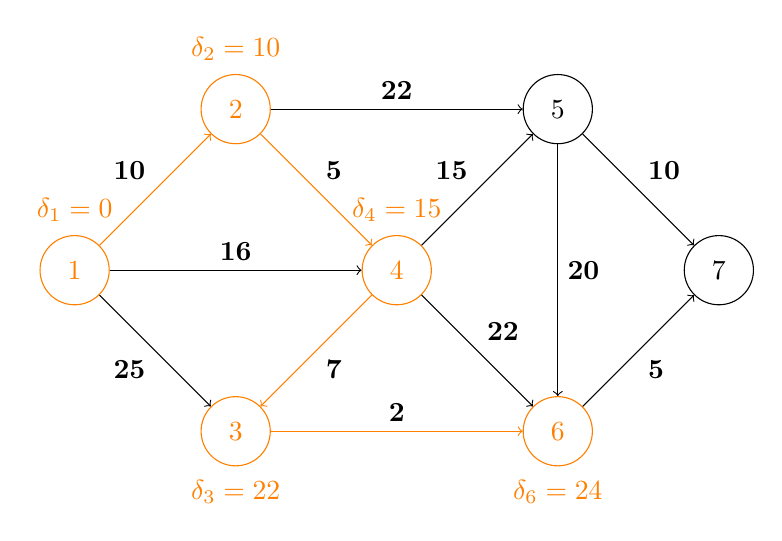
\begin{tikzpicture}[node distance = 2 cm , auto]
        %\tikzset{label/.style={midway,font=\small}}
        \node[state,color=orange] (1) {1};
        \node[above= 0.05 cm of 1] {\textbf{\textcolor{orange}{$\delta_1=0$}}};
        \node[state,color=orange] (2) [above right = of 1] {2};
        \node[above= 0.05 cm of 2] {\textbf{\textcolor{orange}{$\delta_2=10$}}};

        \node[state,color=orange] (3) [below right = of 1] {3};
        \node[below = 0.05 cm of 3] {\textbf{\textcolor{orange}{$\delta_3=22$}}};
        \node[state,color=orange] (4) [below right = of 2] {4};
        \node[above= 0.05 cm of 4] {\textbf{\textcolor{orange}{$\delta_4=15$}}};
        \node[state] (5) [above right = of 4] {5};
        \node[state,color=orange] (6) [below right = of 4] {6};
        \node[below = 0.05 cm of 6] {\textbf{\textcolor{orange}{$\delta_6=24$}}};
        \node[state] (7) [below right = of 5] {7};

        \draw[->,color=orange] (1) edge[color=orange] node[color=black] {\textbf{10}} (2);
        \draw[->] (1) edge node[below left] {\textbf{25}} (3);
        \draw[->] (1) edge node {\textbf{16}} (4);

        \draw[->] (2) edge node {\textbf{22}} (5);
        \draw[->,color=orange] (2) edge[color=orange] node[color=black] {\textbf{5}} (4);

        \draw[->,color=orange] (3) edge[color=orange] node[color=black] {\textbf{2}} (6);

        \draw[->] (4) edge node {\textbf{15}} (5);
        \draw[->] (4) edge node {\textbf{22}} (6);
        \draw[->,color=orange] (4) edge[color=orange] node[color=black] {\textbf{7}} (3);

        \draw[->] (5) edge node {\textbf{20}} (6);
        \draw[->] (5) edge node {\textbf{10}} (7);

        \draw[->] (6) edge node[below right] {\textbf{5}} (7);
    \end{tikzpicture}
\end{center}\pagebreak

\subsection*{Itération 5:}
$EM = \{1,2,4,3,6\}$
\subsubsection*{Étape 1:}
On identifie les sommets adjacents non marqués situé les plus près de:
\begin{itemize}
    \item \textbf{(1)} min $\{\}=\infty$
    \item \textbf{(2)} min $\{22\}\: \Rightarrow j_2 = 5$ \\
    \item \textbf{(4)} min $\{22,15\}\: \Rightarrow j_4 =5$ \\
    \item \textbf{(3)} min $\{2\}\: \Rightarrow j_3 =6$ \\
    \item \textbf{(6)} min $\{5\}\: \Rightarrow j_6 = 7$ \\
\end{itemize}
\subsubsection*{Étape 2:}
min $\{ \infty \:,\: \delta_2 +\lambda_{25} \:,\: \delta_4 + \lambda_{45} \:,\: \infty \:,\: \delta_6 + \lambda_{67}\} = $ min $\{\infty \:,\: 10+22\:,\:15+15\:,\: \infty \:,\:24+5\}=29$\\
marquer le sommet $j_6=7$ avec $\delta_7=29$ 
\subsubsection*{Étape 3:}
$EM=\{1,2,4,3,6,7\}$
\subsubsection*{Étape 4:}
$\overline{EM} \neq \emptyset $ , alors on effectue un autre itération
\begin{center}
    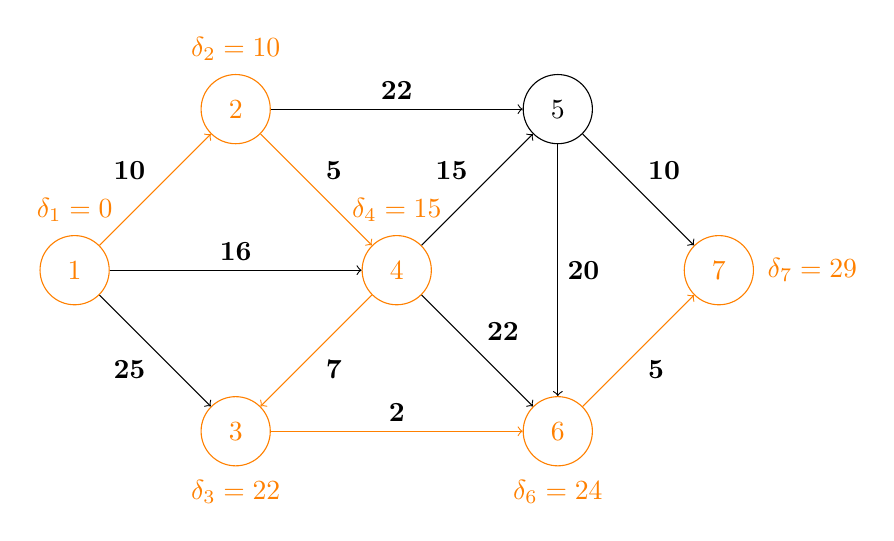
\begin{tikzpicture}[node distance = 2 cm , auto]
        %\tikzset{label/.style={midway,font=\small}}
        \node[state,color=orange] (1) {1};
        \node[above= 0.05 cm of 1] {\textbf{\textcolor{orange}{$\delta_1=0$}}};
        \node[state,color=orange] (2) [above right = of 1] {2};
        \node[above= 0.05 cm of 2] {\textbf{\textcolor{orange}{$\delta_2=10$}}};

        \node[state,color=orange] (3) [below right = of 1] {3};
        \node[below = 0.05 cm of 3] {\textbf{\textcolor{orange}{$\delta_3=22$}}};
        \node[state,color=orange] (4) [below right = of 2] {4};
        \node[above= 0.05 cm of 4] {\textbf{\textcolor{orange}{$\delta_4=15$}}};
        \node[state] (5) [above right = of 4] {5};
        \node[state,color=orange] (6) [below right = of 4] {6};
        \node[below = 0.05 cm of 6] {\textbf{\textcolor{orange}{$\delta_6=24$}}};
        \node[state,color=orange] (7) [below right = of 5] {7};
        \node[right = 0.05 cm of 7] {\textbf{\textcolor{orange}{$\delta_7=29$}}};


        \draw[->,color=orange] (1) edge[color=orange] node[color=black] {\textbf{10}} (2);
        \draw[->] (1) edge node[below left] {\textbf{25}} (3);
        \draw[->] (1) edge node {\textbf{16}} (4);

        \draw[->] (2) edge node {\textbf{22}} (5);
        \draw[->,color=orange] (2) edge[color=orange] node[color=black] {\textbf{5}} (4);

        \draw[->,color=orange] (3) edge[color=orange] node[color=black] {\textbf{2}} (6);

        \draw[->] (4) edge node {\textbf{15}} (5);
        \draw[->] (4) edge node {\textbf{22}} (6);
        \draw[->,color=orange] (4) edge[color=orange] node[color=black] {\textbf{7}} (3);

        \draw[->] (5) edge node {\textbf{20}} (6);
        \draw[->] (5) edge node {\textbf{10}} (7);

        \draw[->,color=orange] (6) edge[color=orange] node[below right,color=black] {\textbf{5}} (7);


    \end{tikzpicture}
\end{center}
\pagebreak

\subsection*{Itération 6:}
$EM = \{1,2,4,3,6\}$
\subsubsection*{Étape 1:}
On identifie les sommets adjacents non marqués situé les plus près de:
\begin{itemize}
    \item \textbf{(1)} min $\{\}=\infty$
    \item \textbf{(2)} min $\{22\}\: \Rightarrow j_2 = 5$ 
    \item \textbf{(4)} min $\{22,15\}\: \Rightarrow j_4 =5$ 
    \item \textbf{(3)} min $\{\}= \infty$
    \item \textbf{(6)} min $\{\}= \infty$
    \item \textbf{(7)} min $\{\}= \infty$
\end{itemize}
\subsubsection*{Étape 2:}
min $\{ \infty \:,\: \delta_2 +\lambda_{25} \:,\: \delta_4 + \lambda_{45} \:,\: \infty \:,\:\infty \:,\:\infty \} = $ min $\{\infty \:,\: 10+22\:,\:15+15\:,\: \infty \:,\:\infty \:,\:\infty \:,\:\infty\}=30$\\
marquer le sommet $j_4=5$ avec $\delta_5=30$ 
\subsubsection*{Étape 3:}
$EM=\{1,2,4,3,6,7,5\}$
\subsubsection*{Étape 4:}
$\overline{EM} = \emptyset $ , alors on arrête 

\begin{center}
    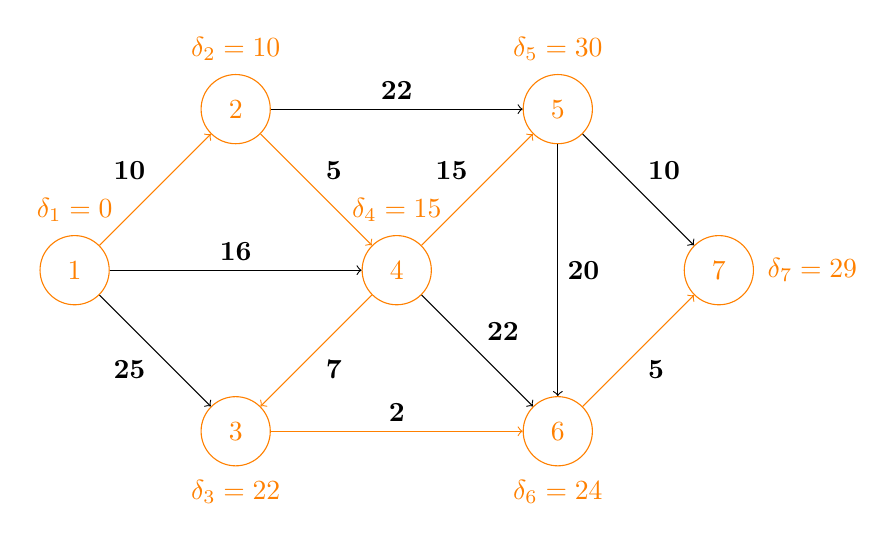
\begin{tikzpicture}[node distance = 2 cm , auto]
        %\tikzset{label/.style={midway,font=\small}}
        \node[state,color=orange] (1) {1};
        \node[above= 0.05 cm of 1] {\textbf{\textcolor{orange}{$\delta_1=0$}}};
        \node[state,color=orange] (2) [above right = of 1] {2};
        \node[above= 0.05 cm of 2] {\textbf{\textcolor{orange}{$\delta_2=10$}}};

        \node[state,color=orange] (3) [below right = of 1] {3};
        \node[below = 0.05 cm of 3] {\textbf{\textcolor{orange}{$\delta_3=22$}}};
        \node[state,color=orange] (4) [below right = of 2] {4};
        \node[above= 0.05 cm of 4] {\textbf{\textcolor{orange}{$\delta_4=15$}}};
        \node[state,color=orange] (5) [above right = of 4] {5};
        \node[above= 0.05 cm of 5] {\textbf{\textcolor{orange}{$\delta_5=30$}}};

        \node[state,color=orange] (6) [below right = of 4] {6};
        \node[below = 0.05 cm of 6] {\textbf{\textcolor{orange}{$\delta_6=24$}}};
        \node[state,color=orange] (7) [below right = of 5] {7};
        \node[right = 0.05 cm of 7] {\textbf{\textcolor{orange}{$\delta_7=29$}}};


        \draw[->,color=orange] (1) edge[color=orange] node[color=black] {\textbf{10}} (2);
        \draw[->] (1) edge node[below left] {\textbf{25}} (3);
        \draw[->] (1) edge node {\textbf{16}} (4);

        \draw[->] (2) edge node {\textbf{22}} (5);
        \draw[->,color=orange] (2) edge[color=orange] node[color=black] {\textbf{5}} (4);

        \draw[->,color=orange] (3) edge[color=orange] node[color=black] {\textbf{2}} (6);

        \draw[->,color=orange] (4) edge[color=orange] node[color=black] {\textbf{15}} (5);
        \draw[->] (4) edge node {\textbf{22}} (6);
        \draw[->,color=orange] (4) edge[color=orange] node[color=black] {\textbf{7}} (3);

        \draw[->] (5) edge node {\textbf{20}} (6);
        \draw[->] (5) edge node {\textbf{10}} (7);

        \draw[->,color=orange] (6) edge[color=orange] node[below right,color=black] {\textbf{5}} (7);


    \end{tikzpicture}
\end{center}
\pagebreak

\section*{Question 3}
\subsection*{(a)}
Pour trouver la matrice de coût, on utilise la formule suivante:
$$c_{ik}=\sum_{j=1,2,3,4} q_{ij} \times d_{}$$
soit $\pi$ une matrice de coût de taille $4\times 4$:

\small
\begin{center}
$$\pi=\begin{pmatrix}
10 \times 50 + 7 \times 30 + 0 \times 70 + 11 \times 100 & 10 \times 50 + 7 \times 30 + 0 \times 50 + 11 \times 60 &  10 \times 95 + 7 \times 55 + 0 \times 25 + 11 \times 55 & 1180 \\
2 \times 50 +30 + 8\times70+4\times100 & 770 & 665 & 695 \\
4 \times 50 +9 \times 30 + 6\times70+0\times100  & 770 & 1025 & 1095 \\
3 \times 50 +5\times30 + 2\times70+7\times100  & 820 & 995 & 745 
\end{pmatrix}$$

$$\pi=\begin{pmatrix}
1810 & 1370 & 1940 & 1180 \\
1090 & 770 & 665 & 695\\
890 & 770 & 1025 & 1095\\
1140 & 820 & 995 & 745

\end{pmatrix}$$

\end{center}

\normalsize
\subsection*{(b)}
\subsubsection*{Étape 1:} Identifier le coût minimal de chaque ligne et le soustraire de chaque élément de la ligne. On obtient la matrice suivante: 
% two matrices side by side

$$\pi=\begin{pmatrix}
1810 & 1370 & 1940 & \textcolor{red}{1180} \\
1090 & 770 & \textcolor{red}{665} & 695\\
890 & \textcolor{red}{770} & 1025 & 1095\\
1140 & 820 & 995 & \textcolor{red}{745}
\end{pmatrix}
\Rightarrow
\begin{pmatrix}
    630 & 190 & 760 & 0 \\
    425 & 105 & 0 & 30\\
    120 & 0 & 255 & 325\\
    395 & 75 & 250 & 0
\end{pmatrix}$$
\subsubsection*{Étape 2:} Identifier le coût minimal de chaque colonne et le soustraire de chaque élément de la colonne. On obtient la matrice suivante:

$$\pi=\begin{pmatrix}
630 & 190 & 760 & \textcolor{red}{0}  \\
425 & 105 & \textcolor{red}{0} & 30\\
\textcolor{red}{120} & \textcolor{red}{0}  & 255 & 325\\
395 & 175 & 250 & \textcolor{red}{0} 
\end{pmatrix}
\Rightarrow
\begin{pmatrix}
510 & 190 & 760 & 0 \\
305 & 105 & 0 & 30\\
0 & 0 & 255 & 325\\
275 & 75 & 250 & 0
\end{pmatrix}$$

\subsubsection*{Étape 3:}Determiner si une affectation de coût 0 est possible.
   % add stiketrough to the lines 2,3 and column 4
$$\begin{pmatrix}
510 & 190 & 760 & 0 \\
305 & 105 & 0 & 30\\
0 & 0 & 255 & 325\\
275 & 75 & 250 & 0
\end{pmatrix}$$

Nous avons besoin de 3 lignes pour couvrir tout les 0  et 3 étant inférieur à 4, nous continuons car il est impossible d'obtenir une affectation de coût 0. 

\subsubsection*{Étape 4:} Ajouter des 0 dans la matrice des coûts : \\
\begin{enumerate}
    \item Identifier le plus petit coût non affecté couvert par une ligne ou une colonne $\Rightarrow$ 75 
    \item soustraire ce coût à chaque élément non couvert par une ligne ou une colonne 
    \item Ajouter ce coût à chaque élément couvert par une ligne et une colonne 
\end{enumerate}
$$\begin{pmatrix}
510 & 190 & 760 & 0 \\
305 & 105 & 0 & 30\\
0 & 0 & 255 & 325\\
275 & \textcolor{red}{75} & 250 & 0
\end{pmatrix}
\Rightarrow
\begin{pmatrix}
    435 & 115 & 685 & 0 \\
    305 & 105 & 0 & 105\\
    0 & 0 & 255 & 400\\
    200 & 0 & 175 & 0
\end{pmatrix}$$

\subsubsection*{Étape 5:} Répéter l'étape 3 et 4 jusqu'à ce qu'une affectation de coût 0 soit possible.
$$\begin{pmatrix}
    435 & 115 & 685 & 0 \\
    305 & 105 & 0 & 105\\
    0 & 0 & 255 & 400\\
    200 & 0 & 175 & 0
\end{pmatrix}$$
Nous avons besoin de 4 lignes pour couvrir tout les 0  et 3 étant inférieur à 4, une affectation de coût 0 est possible.\\

on identifie l'affectation de coût 0 :
$$\begin{pmatrix}
    435 & 115 & 685 & 0 \\
    305 & 105 & 0 & 105\\
    0 & 0 & 255 & 400\\
    200 & 0 & 175 & 0
\end{pmatrix}$$

Ceci nous donne l'affectation suivante dans la matrice des coûts initiale:
$$\pi=\begin{pmatrix}
1810 & 1370 & 1940 & \textcolor{red}{1180} \\
1090 & 770 & \textcolor{red}{665} & 695\\
\textcolor{red}{890} & 770 & 1025 & 1095\\
1140 & \textcolor{red}{820} & 995 & 745
\end{pmatrix}$$

\begin{itemize}
    \item Affecter la machine 1 à l'emplacement d 
    \item Affecter la machine 2 à l'emplacement c
    \item Affecter la machine 3 à l'emplacement a 
    \item Affecter la machine 4 à l'emplacement b 
\end{itemize}

\textbf{Coût total} = 1180 + 665 + 890 + 820 = 3555




\section*{Question 4}
\begin{center}
\begin{tikzpicture}[node distance=1.3cm,auto]
    %center the state at the top ceanter of the page
    \node[state] (1) {1};
    \node[state] (2) [below= of 1] {2};
    \node[state] (3) [below left = of 2] {3};
    \node[state] (4) [below right = of 2] {4};
    \node[state] (5) [below = of 4] {5};
    \node[state] (6) [below = of 5] {6};
    \node[state] (7) [right = of  5] {7};
    \node[state] (8) [below = of  7] {8};
    \node[state] (9) [below = of  8] {9};
    \node[state] (10) [below = of  9] {10};
    \node[state] (11) [below = of  10] {11};
    \node[state] (12) [below = of  11] {12};

    \draw[->] (1) edge node[left] {A} (2);
    \draw[->] (1) edge node[right] {2} (2);

    \draw[->] (2) edge node[left] {B} (3);
    \draw[->] (2) edge node[right] {14} (3);

    % 2 to 4
    \draw[->] (2) edge node[left] {C} (4);
    \draw[->] (2) edge node[right] {14} (4);

    % 4 to 5
    \draw[->] (4) edge node[left] {D} (5);
    \draw[->] (4) edge node[right] {3} (5);

    % 5 to 6
    \draw[->] (5) edge node[left] {F} (6);
    \draw[->] (5) edge node[right] {14} (6);

    % 5 to 7
    \draw[->] (5) edge node[above] {J} (7);
    \draw[->] (5) edge node[below] {7} (7);

    % 6 to 9 
    \draw[->] (6) edge node[left] {G} (9);
    \draw[->] (6) edge node[right] {1} (9);

    % 5 to 9 
    \draw[->] (5) edge node[left] {E} (9);
    \draw[->] (5) edge node[right] {70} (9);

    % 5 to 10 
    \draw[->] (5) edge[bend right, out = 300 , in=240] node[left] {H} (10);
    \draw[->] (5) edge[bend right, out = 300 , in=240] node[right] {1} (10);

    % 5 to 11
    \draw[->] (5) edge[bend right , out=270 , in=270] node[left] {I} (11);
    \draw[->] (5) edge[bend right , out=270 , in=270] node[right] {7} (11);

    % 7 to 8
    \draw[->] (7) edge node[left] {K} (8);
    \draw[->] (7) edge node[right] {14} (8);

    % 8 to 9
    \draw[->] (8) edge node[left] {L} (9);
    \draw[->] (8) edge node[right] {1} (9);

    % 9 to 10
    \draw[->] (9) edge node[left] {M} (10);
    \draw[->] (9) edge node[right] {1} (10);

    % 10 to 11
    \draw[->] (10) edge node[left] {N} (11);
    \draw[->] (10) edge node[right] {1} (11);

    % 11 to 12
    \draw[->] (11) edge node[left] {O} (12);
    \draw[->] (11) edge node[right] {1} (12);

\end {tikzpicture}
\end{center}

\begin{center}
\begin{table}[]
\caption{Temps le plus tard} \label{tab:Temps le plus tard}
    \begin{center}
        \begin{tabular}{|c|c|c|c|}
            \hline
            Étape i & $j \in p_i$ & $LT_j-t_{ij}$ & $LT_i$ \\
            \hline
            12       & -           & -             & 92     \\
            11       & 12          & 92-1          & 91     \\
            10       & 11          & 91-1          & 90     \\
            9        & 10          & 90-1          & 89     \\
            8        & 9           & 89-1          & 88     \\
            7        & 8           & 88-14         & 74     \\
            6        & 9           & 89-1          & 88     \\
            5        & 6           & 88-14         &        \\
                     & 7           & 74-7          &        \\
                     & 9           & 89-70         & 19     \\
                     & 10          & 90-1          &        \\
                     & 11          & 91-7          &        \\
            
            4        & 5           & 19-3          & 16     \\
            3        & 4           & 16-0          & 16     \\
            2        & 3           & 16-14         & 2      \\
            2        & 4           & 16-14         &        \\
            1        & 2           & 2-2           & 0      \\
            \hline
                                                     
                        
                                        
        \end{tabular}
    \end{center}
\end{table}

\begin{table}[]
    \caption{Temps le plus tôt} \label{tab:Temps le plus tard}
    \begin{center}
        \begin{tabular}{|c|c|c|c|}
            \hline
            Étape i & $j \in B_i$ & $ET_j+t_{ji}$ & $ET_i$ \\
            \hline
            1        & -           & -             & 0      \\
            2        & 1          & 0+12          & 2      \\
            3        & 2          & 2+14          & 16     \\
            4        & 2          & 2+14          & 16     \\
                     & 3          & 2+0           &        \\
            5        & 4           & 16+3          & 19     \\
            6        & 5           & 19+14         & 33     \\
            7        & 5           & 19+7          & 26     \\
            8        & 7           & 26 +14        & 40     \\
            9        & 5           & 19+70         & 89     \\
                     & 6          & 33+1          &        \\
                     & 8          & 40+1          &        \\
            10       & 5           & 19+1          & 90     \\
                     & 9           & 89+1          &        \\
            11       & 5           & 19+7          & 91     \\
                     & 10           & 90+1          &        \\
            12       & 11           & 91+1          & 92     \\
            \hline
                                                     
                        
                                        
        \end{tabular}
    \end{center}
\end{table}

\begin{table}[]
    \caption{Écarts} \label{tab:Temps le plus tard}
    \begin{center}
        \begin{tabular}{|c|c|c|}
           \hline
           Tâches & $LT_j-(ET_i+t_{ij})$ & Écart \\
           \hline 
           (1,2) & $2-(0+2)$ & 0 \\

           (2,3) & $16-(2+14)$ & 0 \\

           (2,4) & $16-(2+14)$ & 0 \\

           (3,4) & $16-(16+0)$ & 0 \\

           (4,5) & $19-(16+3)$ & 0 \\

           (5,6) & $88-(19+14)$ & 55 \\
           
           (5,7) & $76-(19+7)$ & 48 \\
           
           (5,9) & $89-(19+70)$ & 0 \\
           
           (5,10) & $90-(19+1)$ & 70 \\

           
           (5,11) & $91-(19+7)$ & 65 \\

           (6,9) & $89-(33+1)$ & 55 \\
           
           (7,8) & $88 - (26 + 14)$ & 48 \\
           
           (8,9) & $89-(40+1)$ & 48 \\
           
           (9,10) & $90-(89+1)$ & 0 \\
           
           (10,11) & $91 - (90 + 1)$ & 0 \\
           
           (11,12) & $92-(91+1)$ & 0 \\


            \hline
                                                     
                        
                                        
        \end{tabular}
    \end{center}
\end{table}
\end{center}

\end{document}
